% !Mode:: "TeX:UTF-8"
%%  本模板推荐以下方式编译:
%%
%%     1. PDFLaTeX[推荐]
%%  注意:
%%   1. 文件默认的编码为 UTF-8 对于windows,请选用支持UTF-8编码的编辑器。
%%   2. 若是模板有什么问题,请及时与我们取得联系,Email:latexstudio@qq.com。
%%   3. 可以到  https://wenda.latexstudio.net 提问
%%   4. 请安装 最新版本的 TeXLive 地址:https://www.latexstudio.net/page/texsoftware/

\documentclass{apmcmthesis}

\usepackage{url}

%%%%%%%%%%%%填写相关信息%%%%%%%%%%%%%%%%%%%%%%%%%%
\tihao{A}                            %选题
\baominghao{2020230010136}           %报名号

\begin{document}

\pagestyle{frontmatterstyle}

\begin{abstract}
  With laser, the hatch tool of laser marking machine can be used to realize the work of making two-dimensional graphics. However, the selection and layout of hatch methods and paths greatly affect the difficulty and efficiency of incubation. The hatch problem of the laser marking machine on the two-dimensional closed graph can be equivalent to the problem of filling the two-dimensional closed curvilinear polygon with the curves connected by scattered points. Here, we provide two Python-based filling algorithms. They respectively correspond the zigzag hatch and the contour parallel hatch. Both of these two algorithms utilize vectors to the greatest extent on the basis of inward shrinking of the initial graphics to process the graphics lattice data, and use the distance between two points and the argument of vector as the basis for determining. Importantly, the algorithm automatically filters the lattice data at the sharp points of the figure after rational simplification, optimizes the shrinking of the arc with a very small radius of curvature. It also can ensure that the graphics formed after filtering can meet the requirements. This method breaks the limitation of the traditional algorithm that can only handle simple geometric figures. It provides the possibility to deal with complex curve polygons, and optimize the laser marking machine’s refined processing of complex graphics. Meanwhile, we avoid solving a large number of linear equations in the algorithm and improve its efficiency. However, because of the filtering of the lattice, the graphics we get may have some unexpected deformation. Therefore, we still need some extra program to adjust it. 
  \keywords{Python\quad  filling algorithm\quad   vector\quad  zigzag hatch\quad  contour parallel hatch}
\end{abstract}



\newpage
%目录
\tableofcontents


\newpage
\pagestyle{mainmatterstyle}
\setcounter{page}{1}
\section{Introduction}
The sharpest knife, laser, has been widely used to mark specified 2D-compound curve graph. Efficiency is an important indicator for this craft. To maximize the efficiency, we need to make the hatch curves generated automatically and quickly by laser marking machine keep parallel to the boundary lines of the figures, and distribute evenly.\cite{4}



\subsection{Problem Restatement}
  The curve used by laser etching has a certain width. In order to simplify the calculation, we approximate it to a one-dimensional curve, and set the spacing of the curve to achieve the filling effect. Taking into account the moving efficiency of the robotic arm in actual industrial production, the curve used to fill the graph must be as continuous as possible. Based on the above discussion, we can equate the problem as the optimal solution for filling a two-dimensional curve polygon with a continuous curve.


\subsection{Previous Work}
  In previous work, we have learned that there has been a work of depicting a vector diagram by calculating basic data through DSP. In the processing of bitmaps, due to the large storage space occupied by bitmap files, a small amount of pixel data is selected according to the set resolution during the processing of the marking software. Such processing greatly reduces the amount of marking data of the bitmap file and improves its marking speed. Increasing the resolution of the picture can improve the fineness of the graphic marking, but due to the limitation of the scanning speed, the marking time increases accordingly.


\subsection{Problem Solving Strategies}
For the two hatching methods mentioned in the question, we originally proposed two different general algorithm. They can solve such problems universally.
For the zigzag hatching, we first indent the graphics formed by the original lattice. And by finding the extreme points of the graphics, a dividing line parallel to the x-axis is made according to the traversal direction to intersect the graphics at one point. Therefore, we divide the entire graphics into a number of areas. Finally, we do zigzag hatching from top to bottom in each partition.
For the contour parallel hatch, we will iterate the steps of indentation. In the process of iteration, we will remove points that will cause overlap in the coverage area. When the last curve generated by the iteration is about to cross, stop the iteration and partition the area formed by the last curve. Finally, we continue to iterate until the filling accuracy requirement is reached.

\section{The Description of the algorithms}
\subsection{How do we use algorithms to implement the whole process?}

\begin{itemize}
  \item
  \item
  \item
\end{itemize}


\subsection{The Reasonableness of approximating}
1)           :\par
2) From the perspective of the      :\par
3) Compromise:

\subsection{The local optimization and the overall optimization}


\begin{itemize}
  \item
  \item
  \item Virtually:
\end{itemize}


\subsection{Algorithmic Complexity}



\section{Models}
\subsection{Basic Model}


\subsubsection{Terms, Definitions and Symbols}
The signs and definitions are mostly generated from queuing theory.


\subsubsection{Assumptions}


\subsubsection{The Foundation of Model}
1) The utility function

\begin{itemize}
  \item The cost of       :
  \item The loss of       :
  \item The weight of each aspect:
  \item Compromise:
\end{itemize}



\begin{figure}[!ht]
  \centering
  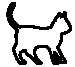
\includegraphics[width=3cm]{cat}  \quad  
\includegraphics[width=5cm]{gongzhonghao}
  \caption{\CJK{UTF8}{gbsn}{关注我们公众号,学习更多知识}}\label{cat1}
\end{figure}



3) The overall optimization and the local optimization

\begin{itemize}
  \item The overall optimization:
  \item The local optimization:
  \item The optimal number of        :
\end{itemize}



\subsubsection{Solution and Result}
1) The solution of the integer programming:
2) Results:
\subsubsection{Analysis of the Result}
\begin{itemize}
  \item Local optimization and overall optimization:
  \item Sensitivity: The result is quite sensitive to the change of the three parameters
  \item
  \item Trend:
  \item Comparison:
\end{itemize}
\subsubsection{Strength and Weakness}

\begin{description}
  \item[Strength:] The Improved Model aims to make up for the neglect of         . The result seems to declare that this model is more reasonable than the Basic Model and much more effective than the existing design.
  \item[Weakness:] Thus the model is still an approximate on a large scale. This has doomed to limit the applications of it.
\end{description}

\section{Conclusions}

\subsection{Conclusions of the problem}
\begin{itemize}
  \item
  \item
  \item
  \item
\end{itemize}
\subsection{Methods used in our models}
\begin{itemize}
  \item
  \item
  \item
  \item
\end{itemize}
\subsection{Applications of our models}
\begin{itemize}
  \item
  \item
  \item
  \item
\end{itemize}
\section{Future Work}
\subsection{Ideas to solve existing problems}
Zigzag, as the most common hatching method at present, has many sharp turns. For shapes with complex borders or hollow, this disadvantage will be very obvious.The contour parallel algorithm can avoid too many sharp turns, but it leads to more contours and the contours are not connected. For the problems of these two hatching methods, we can use the Fermat spiral filling used in 3D printing to solve it. The Fermat spiral consists of two intertwined sub-helices, one inward and the other outward. The Fermat spiral has three advantages:
1) Similar to the contour parallel hatch, the Fermat spiral only has a sharp turn at the center.
2) Some Fermat spirals can continuously fill the 2D area; traditional spirals are either inward or outward, and Fermat spirals are both inward and outward, and can meet at the boundary.
3) To facilitate the connection between the spirals, the start and end nodes of the Fermat spiral can be selected arbitrarily at the boundary.



\subsection{Optimization of performance and efficiency}


\subsection{Realization of practical industrial applications}









%参考文献
\begin{thebibliography}{9}%宽度9
  \bibitem{1} Author, Title, Place of Publication: Press, Year of publication.
  \bibitem{2} author, paper name, magazine name, volume number: starting and ending
  page number, year of publication.
  \bibitem{3} author, resource title, web site, visit time (year, month, day).
  \bibitem{bib:one} \LaTeX{}\CJK{UTF8}{gbsn}{资源和技巧学习} \url{https://www.latexstudio.net}
  \bibitem{bib:two} \LaTeX{}\CJK{UTF8}{gbsn}{问题交流网站} \url{https://wenda.latexstudio.net}
  \bibitem{bib:two} \CJK{UTF8}{gbsn}{模板库维护} \url{https://github.com/latexstudio/APMCMThesis}
  \bibitem{4} Kaposi, M. “IDIOPATHISCHES MULTIPLES PIGMENTSARKOM DER HAUT.” Wiener Klinische Wochenschrift, vol. 4, no. 2, 1872, pp. 265–273.
\end{thebibliography}

\newpage
%附录

\section{Appendix}
\begin{lstlisting}[language=matlab,caption={The matlab Source code of Algorithm}]
kk=2;[mdd,ndd]=size(dd);
while ~isempty(V)
[tmpd,j]=min(W(i,V));tmpj=V(j);
for k=2:ndd
[tmp1,jj]=min(dd(1,k)+W(dd(2,k),V));
tmp2=V(jj);tt(k-1,:)=[tmp1,tmp2,jj];
end
tmp=[tmpd,tmpj,j;tt];[tmp3,tmp4]=min(tmp(:,1));
if tmp3==tmpd, ss(1:2,kk)=[i;tmp(tmp4,2)];
else,tmp5=find(ss(:,tmp4)~=0);tmp6=length(tmp5);
if dd(2,tmp4)==ss(tmp6,tmp4)
ss(1:tmp6+1,kk)=[ss(tmp5,tmp4);tmp(tmp4,2)];
else, ss(1:3,kk)=[i;dd(2,tmp4);tmp(tmp4,2)];
end;end
dd=[dd,[tmp3;tmp(tmp4,2)]];V(tmp(tmp4,3))=[];
[mdd,ndd]=size(dd);kk=kk+1;
end; S=ss; D=dd(1,:);
 \end{lstlisting}
\begin{lstlisting}[language=c,caption={The lingo source code}]
kk=2;
[mdd,ndd]=size(dd);
while ~isempty(V)
    [tmpd,j]=min(W(i,V));tmpj=V(j);
for k=2:ndd
    [tmp1,jj]=min(dd(1,k)+W(dd(2,k),V));
    tmp2=V(jj);tt(k-1,:)=[tmp1,tmp2,jj];
end
    tmp=[tmpd,tmpj,j;tt];[tmp3,tmp4]=min(tmp(:,1));
if tmp3==tmpd, ss(1:2,kk)=[i;tmp(tmp4,2)];
else,tmp5=find(ss(:,tmp4)~=0);tmp6=length(tmp5);
if dd(2,tmp4)==ss(tmp6,tmp4)
    ss(1:tmp6+1,kk)=[ss(tmp5,tmp4);tmp(tmp4,2)];
else, ss(1:3,kk)=[i;dd(2,tmp4);tmp(tmp4,2)];
end;
end
    dd=[dd,[tmp3;tmp(tmp4,2)]];V(tmp(tmp4,3))=[];
    [mdd,ndd]=size(dd);
    kk=kk+1;
end;
S=ss;
D=dd(1,:);
 \end{lstlisting}


\end{document}